\documentclass[letterpaper,10pt,onecolumn]{IEEEconf}
% \documentclass[letterpaper,10pt,draftclsnofoot,onecolumn]{IEEEconf}

\usepackage{amsmath,amssymb}
\usepackage{graphicx,color,xspace}
\usepackage[ruled, vlined]{algorithm2e}

\begin{document}

\title{Homework 1 - Prototype selection for nearest neighbor}
\author{Evan Gravelle \quad \quad October 13, 2016}
\maketitle

\section{Prototype Selection Methodology}

My method for prototype selection from MNIST data utilizes $k$-means clustering to group the training data into $k$ clusters. Each cluster's mean is then assigned a label, by performing a nearest neighbor search on the original training data. The set of means with associated labels serves as the set of prototypes.

\section{Pseudocode}

\begin{algorithm}[H]
\SetAlgoLined
\DontPrintSemicolon
\SetKwInOut{Input}{Input}\SetKwInOut{Output}{Output}
\Input{Training set $T$, number of prototypes $m$}
\Output{Prototype set $P$}
\BlankLine
Initialize $P$ randomly from $T$, where $|P| = m$ \\
Assign each $t \in T$ to nearest cluster $p \in P$ \\
Define $Q$ as average distance from point $t \in T$ to assigned cluster $p \in P$ \\
\While{$Q$ has no sufficiently converged}{
\For{$t \in T$}{
Calculate centroid $C_p$ of each cluster \\
Assign $P = \{ C_p \}$ for all $p \in P$\\
Assign $t$ to nearest cluster $p \in P$ \\
Update $Q$
}
}
\For{$p \in P$}{
Assign label of nearest neighbor of $p$ to $P$
}
Return $P$
\caption{Prototype Selection Algorithm}
\end{algorithm}

\section{Experimental}

\begin{center}\label{fig:plot}
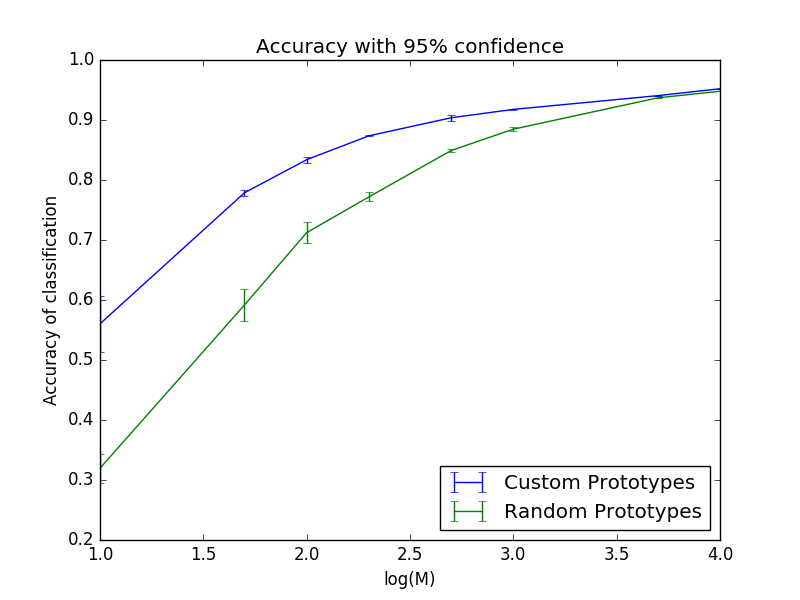
\includegraphics[width=10cm]{errorbars.png}
\end{center}

Three data points were recorded for each value of $m$ under 5000. Only one data point was recorded when $m \in \{5000, 10000 \}$, this is due to the long running time of the algorithm.

\section{Critical Evaluation}

As seen in Figure~\ref{fig:plot}, this method of prototype selection outperforms random prototype selection for all tested values of $m$ between 10 and 10,000. Still, there are potentially multiple avenues for improvement in prototype selection. $k$-means clustering does not use the label during cluster formation, so a constrained version could help, where each point in a cluster the same label. The nearest neighbor of the cluster centroid is used to determine the label for the cluster, when perhaps a higher order nearest neighbor assignment would work better, or some sort of function approximation to assign the label. 

\end{document}